% !TeX encoding=utf8
% !TeX spellcheck = en-US

\chapter{Methods}
Here we describe the data used and detail the implementation. We first examine in detail two methods for link prediction: collaborative filtering using the Jaccard similarity metric and the Triadic Closeness method. We then show how these two methods can be used together in an ensemble predictor using adaptive weights. The data used in this experiment is examined. Finally, implementation is discussed. 

We focus on the link prediction problem for a partially observed network. We assume certain links are missing form the network and attempt to predict the missing link(s), focusing on User-User edges.

\section{Sample Network}
Consider the network shown in figure \ref{thesis_sample_network}. This is a sample network which was randomly generated and does not represent any real world observed data, however we shall refer to this network to demonstrate the techniques used in this project. The sample network contains two types of nodes: Users and Items. Each User can \textit{FOLLOW} other Users. This is represented as a User-User directed edge with the label \textit{:FOLLOWS}. Similarly, Users can express their interest in an Item with the \textit{:LIKES} relationship (or edge). This type of network structure is similar to those observed in social networks (such as Facebook, or Twitter), but also in collaboration networks (such as Github, as we will see in more detail). Since the network has multiple types of nodes and edges it is referred to as a \textbf{multi-modal network}. (CITE GRAPH THEORY / COMPLEX NETWORK BOOK). 

\begin{figure}[H]
  \centering
  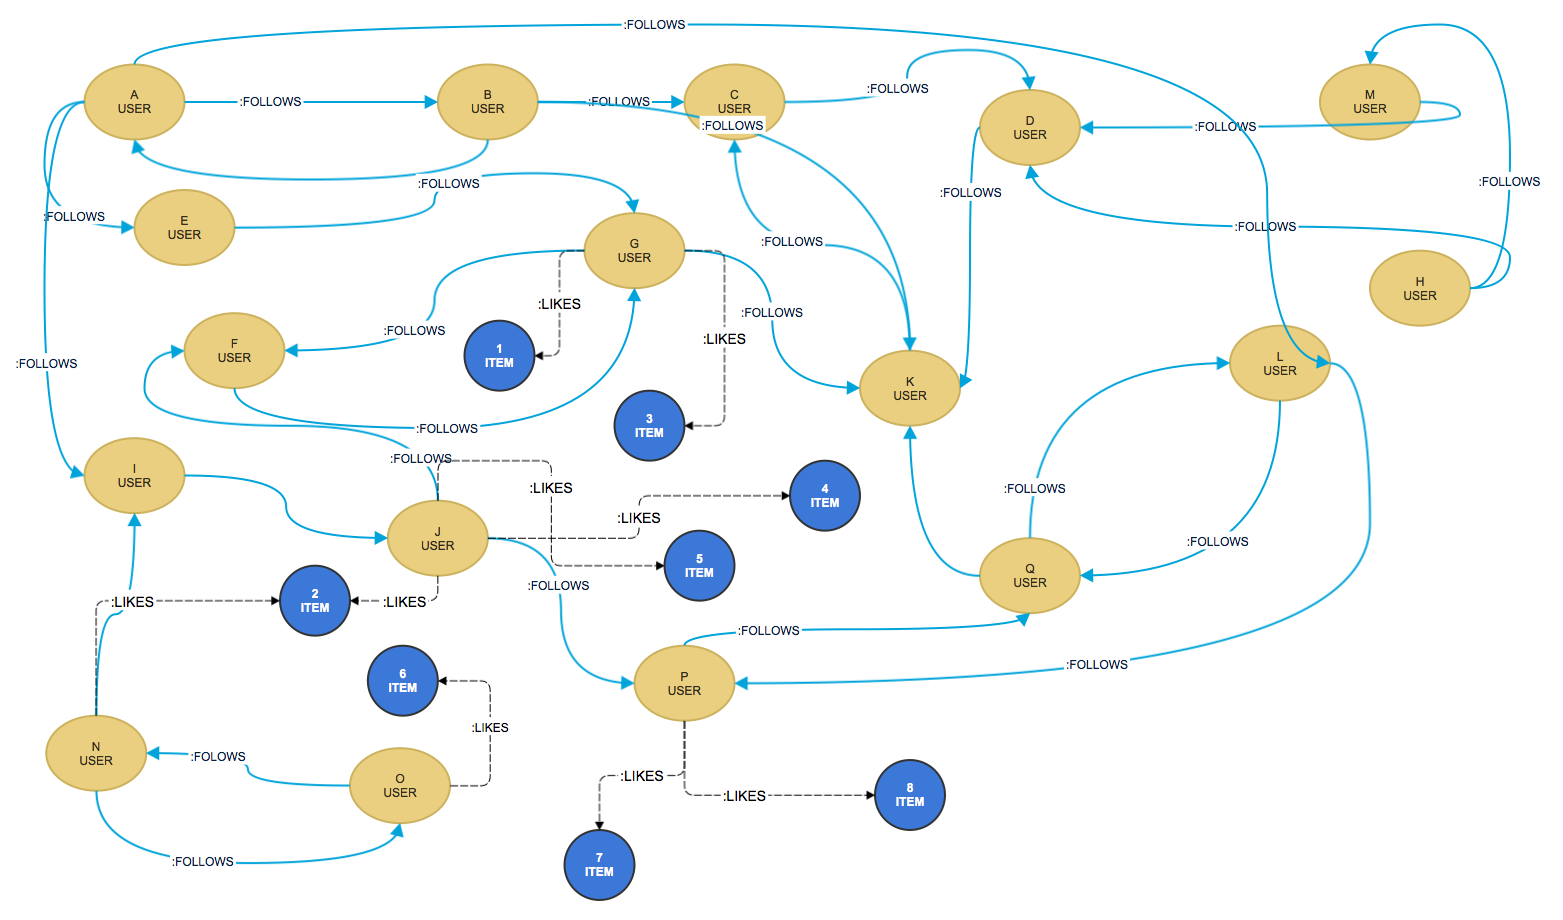
\includegraphics[width=0.75\textwidth]{images/thesis_sample_network_multimodal.png}
  \caption[Sample multi-modal network]{This sample network will be used to demonstrate the methods used for link prediction in this paper. This network demonstrates a random multi-modal network with multiple types of nodes and edges.}
  \label{thesis_sample_network}
\end{figure}

\begin{table}[t]
\caption{Descriptive statistics for sample network}
\label{sample_network_stats}
\vskip 0.15in
\begin{center}
\begin{small}
\begin{sc}
\begin{tabular}{rc}
\hline
Metric & value\\
\hline
Num nodes & 17\\
Num edges & 28\\
Avg degree & 1.67\\
OTHERS & ??\\
\hline
\end{tabular}
\end{sc}
\end{small}
\end{center}
\vskip -0.1in
\end{table}

Some basic descriptive statistics about this sample network are shown in Table \ref{sample_network_stats}. 

\section{Algorithms}

For illustrative purposes we will work through three examples of link prediction algorithms for the sample network shown above. First, using the collaborative filtering method with the Jaccard similarity metric. We will use User-Item edges to identify similar uses and generate recommendations based on those similarities. Next, we walk through the Triadic Closeness method as described in \cite{Schall2014}. Using probabilities observed from triad patterns we will generate link predictions and compare to those created using collaborative filtering. Finaly, we propose a ensemble method that combines collaborative filtering and Triadic Closeness using an adaptive weighting system. In the context of the sample network we focus on predicting User-User \textit{:FOLLOWS} edges only.

For the purposes of the next three sections we will consider link prediction for user J. We proceed through each algorithm manually, ignoring some implementation details for now that will explored in depth in the proceeding section.

\subsection{Collaborative Filtering}
Collaborative filtering is a method of generating recommendations based on the homophily principle: users who are similar are likely to be interested in similar items. It is implemented by finding similar users, based on some similarity metric. \cite{cf} Here we will use User-Item edges as an indication of a User's binary rating of an Item. The Jaccard metric is used to show a proportion of overlapping neighbors

\subsubsection{Similarity Metrics}
The Jaccard index is used to identify similar users. For two users, $a$ and $b$, let $A$ and $B$ denote the sets of all users being followed by $a$ and $b$, respectively. The Jaccard index is therefore as defined in Equation \ref{jaccard}.
\begin{equation}
\label{jaccard}
J(A,B) = \frac{|A \cap B|}{|A \cup B|}
\end{equation}

In this context, Jaccard is defined as the intersection of the Items liked by $a$ and $b$ divided by the union of the items likes by $a$ and $b$. This results in a number between 0 and 1, indicating the strength of similarity between users $a$ and $b$.
 
%\begin{algorithm}[tb]
%
%  \caption{Collaborative Filtering Recommendation}
%   \label{alg:cf}
%\begin{algorithmic}
%   \STATE {\bfseries Input:} Graph $G(V,E)$, vertex $v$, int k
%   
%   \FOR{$i=1$ {\bfseries to} $m-1$}
%   \IF{$x_i > x_{i+1}$} 
%   \STATE Swap $x_i$ and $x_{i+1}$
%   \STATE $noChange = false$
%   \ENDIF
%   \ENDFOR
%  
%\end{algorithmic}
%\end{algorithm}

FIXME: THIS NEEDS TO BE UPDATED FOR NEW DATA MODEL
\begin{algorithm}
\caption{Collaborative filtering algorithm}\label{algo1}
\begin{algorithmic}[1]
\State $input: G(U, E), x, N$ \Comment{explain inputs here}
\State $usersSample \gets getRandomUsers(U,x)$
\State $results \gets \{\}$
\For {$each user in usersSample$}
	\State $validationEdge \gets getRandomEdge(G, user)$
	\State $removeEdge(validationEdge,G)$
	\State fofs $\gets getFOFS(user, G)$
	\State fofRanks $ \gets \{\}$
	\For{each fof in fofs}
		\State j $\gets jaccard(user, fof)$
		fofRanks $\gets results + \{j : fof\}$
	\EndFor
	\State knn $\gets topk(fofRanks, k)$
	\State aggregated $\gets \{\}$
	\For{each kn in knn}
		\State possible $\gets getFollows(kn)$
		\For{each p in possible}
			\If{p in aggregated.keys} $aggregated[p] += 1$ 
				%\State 
			\Else 
				\State $aggregated[p] = 1$
			\EndIf
		\EndFor
	\EndFor
	
	\State $predictions \gets topXSortedByTC(pred, N)$
	\State $hit \gets is validationEdge in predictions?$
	\State $addEdge(validationEdge, G)$
	\State $results \gets results + \{hit, pred, u, v, validation_edge\}$
\EndFor
\State \Return results
\end{algorithmic}
\end{algorithm}

To generate recommendations for user $J$, we first must identify all friend-of-friend nodes, that is nodes that share a neighbor Item in common with $J$. That gives us the set $\{N\}$. Our possible recommendations are now reduced to N. We will now compute the Jaccard similarity metric for the pair $(J, N)$:

\begin{equation}
\label{jaccard}
J(J,N) = \frac{|J \cap N|}{|J \cup N|}
\end{equation}

\begin{equation}
\label{jaccard}
J(J,N) = \frac{|\{Item2\}|}{|\{Item2, Item4, Item5\}|}
\end{equation}

\begin{equation}
\label{jaccard}
J(J,G) = \frac{1}{3}
\end{equation}

We can now predict the edge $J \leftarrow N$ with weight $1/3$. \footnote{If we were interested in predicting User-Item links, we could allow each similar user to \textit{vote} for other Items in which J might have an interest. We now take the top $k$ nodes that have the highest Jaccard score and allow each to vote for new outgoing links to form from $J$. Here we will select $L$ and recommend any outgoing links from $L$ as destination nodes for predicted links emminating from $J$. However, we are only concerned here with User-User edges.}

As you can see, the collaborative filtering link prediction process for a given user $x$ involves finding other users most similar to user $x$, then finding items those similar users are most interested in. In this sense collaborative filtering can be thought of as very similar to k-nearest neighbors, where the distance calculation is based on some similarity metric.

\subsection{Triadic Closeness}
Graph theory proposes the concept of triadic closure, the hypothesis that the creation of an edge between u and v is related to the degree of overlapping neighbors in u and v's respective networks. (CITATION NEEDED and expand on this - see one of the network analysis books I have) The concept of Triadic Closeness is an application of the theory of triadic closure, specifically taking into account the directed nature of social networks. For a given fully observed network, Triadic Closeness can be thought of as the ratio of the number of closed triads to the number of potentially closed triads. \cite{Schall2014}. A triad consists of three nodes $u, z, v$ where edges (ignoring direction) $u,z$ and $z,v$ exist. Edges between $u$ and $v$ may exist, however the concept of triadic closure posits that an implicit connection exists between $u$ and $v$.

\begin{algorithm}
\caption{Triadic Closeness link prediction algorithm}\label{algo_tc}
\begin{algorithmic}[1]
\State $input: G(U, E), x, N$ \Comment{explain inputs here}
\State $usersSample \gets getRandomUsers(U,x)$
\State $results \gets \{\}$
\For {$each user in usersSample$}
	\State $validationEdge \gets getRandomEdge(G, user)$
	\State $removeEdge(validationEdge,G)$
	\State $triads \gets getTriads(user, G)$
	\State $pred \gets \{\}$
	\For {$u, v in triads$}
		\State $tc \gets calcTC(u,v,G)$
		\State $pred \gets pred + \{tc, u, v\}$
	\EndFor
	\State $predictions \gets topXSortedByTC(pred, N)$
	\State $hit \gets is validationEdge in predictions?$
	\State $addEdge(validationEdge, G)$
	\State $results \gets results + \{hit, pred, u, v, validation_edge\}$
\EndFor
\State \Return results
\end{algorithmic}
\end{algorithm}


\begin{figure}[H]
  \centering
  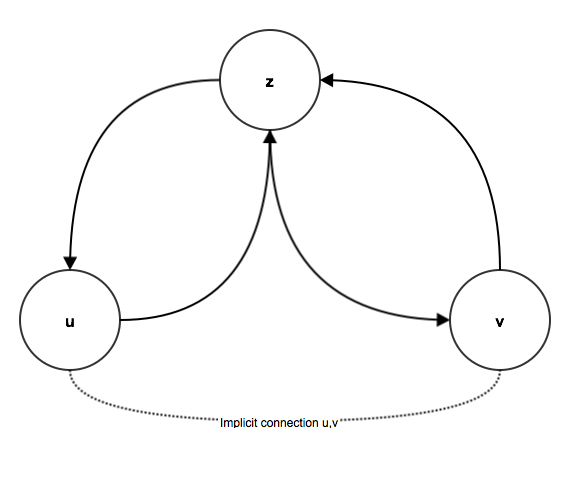
\includegraphics[width=0.4\textwidth]{images/thesis_triad_example.png}
  \caption[closed triad patterns]{A triad is considered to be closed if an edge exists between u and v.}
  \label{thesis_closed_triads}
\end{figure}


In a directed network there are 27 distinct configurations, or patterns that a triad can take on. See (CITATION TABLE of triad patterns). Table \ref{sample_network_freq} shows triad patterns that are open, that is no connection exists between nodes $u$ and $v$. The pattern identifications $(T01, T02...)$ are taken from (CITE PROPERLY) Schall 2013. Any open triad can be closed in one of three possible ways: $u \leftarrow v$, $u \rightarrow v$, or $u \leftrightarrow v$.

INSERT IMAGE OF 3 CLOSED TRIAD PATTERNS 
\begin{figure}[H]
  \centering
  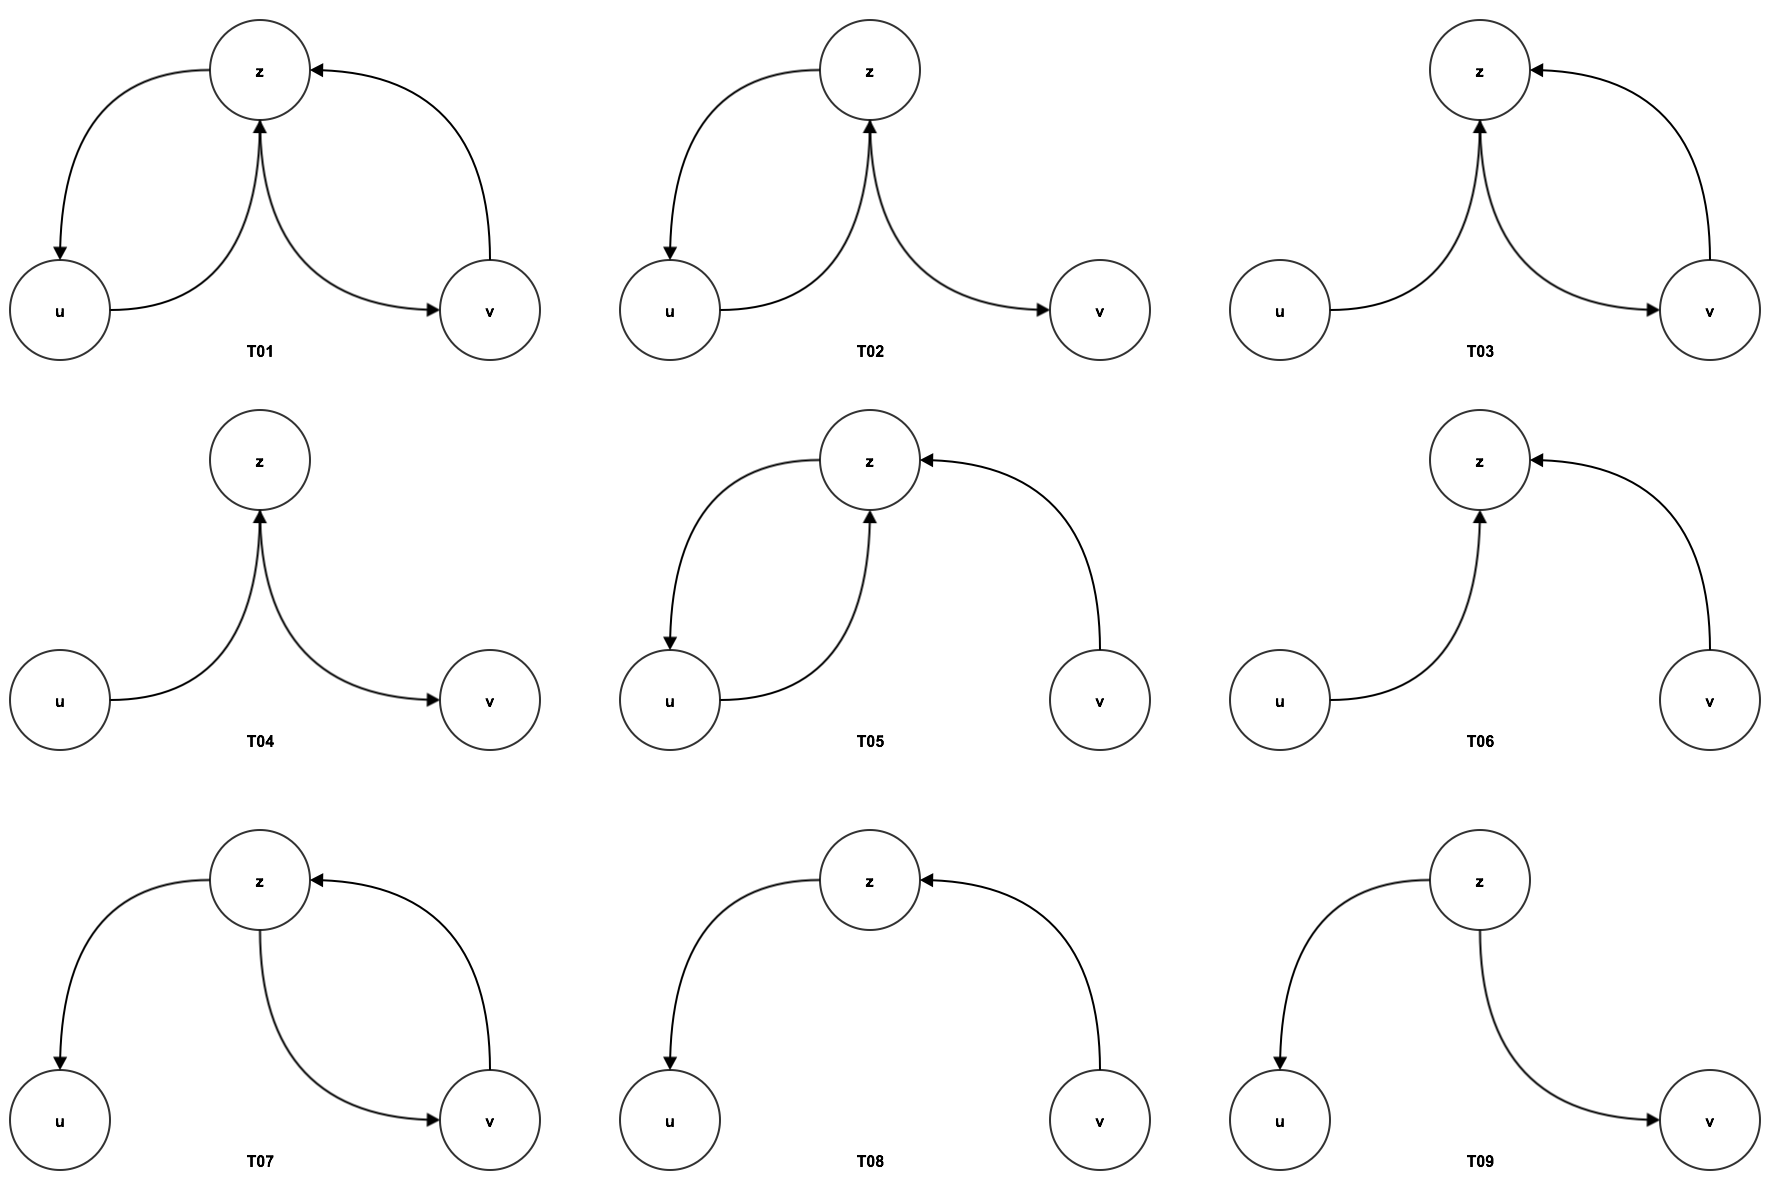
\includegraphics[width=0.75\textwidth]{images/thesis_triad_patterns.png}
  \caption[triad patterns]{All possible open triad patterns are shown. A triad is said to be closed is a connection is established between u and v.}
  \label{thesis_triad_patterns}
\end{figure}

\begin{figure}[H]
  \centering
  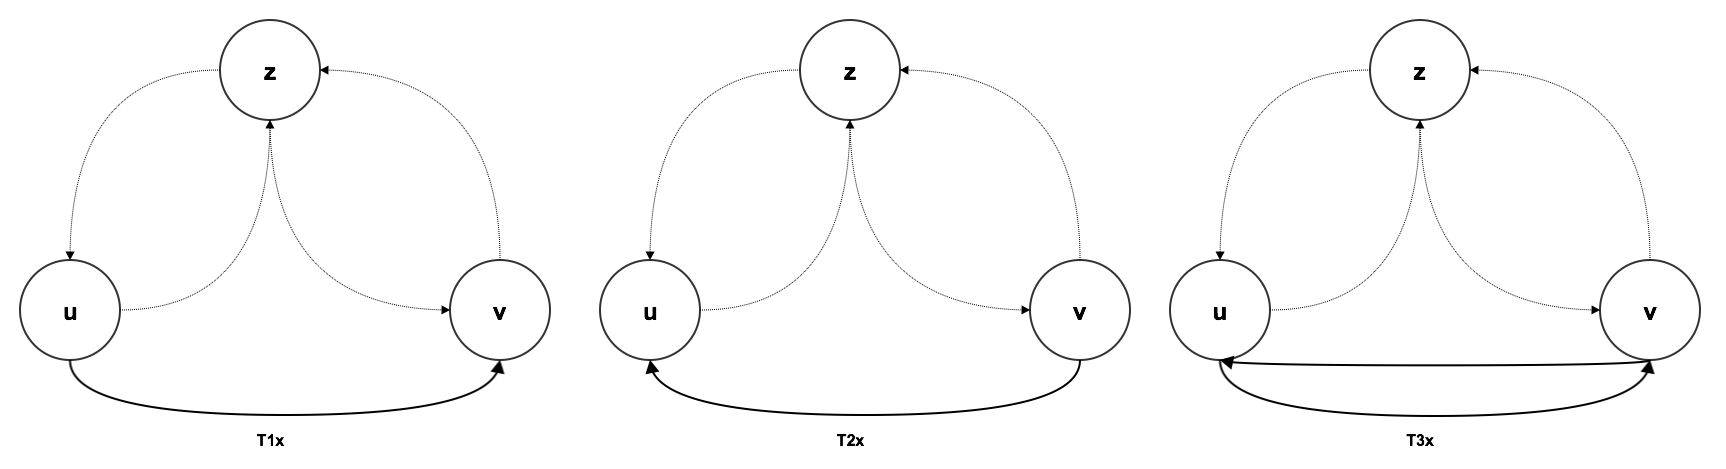
\includegraphics[width=0.75\textwidth]{images/thesis_closed_triads.png}
  \caption[closed triad patterns]{A triad is considered to be closed if an edge exists between u and v.}
  \label{thesis_closed_triads}
\end{figure}

Figure \ref{thesis_closed_triads} shows the three distinct ways in which an open triad can be closed. Either the creation of an edge $u \rightarrow u$, the creation of an edge $u \leftarrow v$, or the creation of two edges $u \rightarrow v$ and $u \leftarrow v$. In terms of the triad pattern id, the first digit indicates if the triad is open (0), closed with an edge $u \rightarrow v$ (1), closed with an edge $u \leftarrow v$ (2), or closed with two edges $u \rightarrow v$ and $u \leftarrow v$ (3). With this nomenclature we are now able to represent each possible triad pattern with a two digit identifier. 

\begin{table}[t]
\caption{Open triad pattern frequency in the sample network shown in Figure CITATION NEEDED}
\label{sample_network_freq}
\vskip 0.15in
\begin{center}
\begin{small}
\begin{sc}
\begin{tabular}{rrccr}
\hline
ID & Pattern & Count \\
\hline
T06 & $u \rightarrow z \leftarrow v $ & 20 \\
T04 &$ u \rightarrow z \rightarrow v$ & 14 \\
T08 & $u \leftarrow z \leftarrow v$ & 14 \\
T02 & $u \leftrightarrow z \rightarrow v$ & 8 \\
T07 & $u \leftarrow z \leftrightarrow v$ & 8 \\
T09 & $u \leftarrow z \rightarrow v$ & 8 \\
T03 & $u \rightarrow z \leftrightarrow v$ & 3 \\
T05 & $u \leftrightarrow z \leftarrow v$ & 3 \\

\hline
\end{tabular}
\end{sc}
\end{small}
\end{center}
\vskip -0.1in
\end{table}

\begin{table}[t]
\caption{Closed triad pattern frequency in the sample network shown in Figure CITATION NEEDED}
\label{sample_network_freq}
\vskip 0.15in
\begin{center}
\begin{small}
\begin{sc}
\begin{tabular}{rrccr}
\hline
ID & Pattern & Count \\
\hline
T18 & $u \leftarrow z \leftarrow v \leftarrow u$ & 3 \\
T14 & $u \rightarrow z \rightarrow v \leftarrow u$ & 2 \\
T16 & $u \rightarrow z \leftarrow v \leftarrow u$ & 2 \\
T19 & $u \leftarrow z \rightarrow v \leftarrow u$ & 2 \\
T15 & $u \leftrightarrow z \leftarrow v \leftarrow u$ & 1 \\
T17 & $u \leftarrow z \leftrightarrow v \leftarrow u$ & 1 \\
T24 & $u \rightarrow z \rightarrow v \rightarrow u$ & 3 \\
T26 & $u \rightarrow z \leftarrow v \rightarrow u$ & 2 \\
T28 & $u \leftarrow z \leftarrow v \rightarrow u$ & 2 \\
T29 & $u \leftarrow z \rightarrow v \rightarrow u$ & 2 \\
T22 & $u \leftrightarrow z \rightarrow v \rightarrow u$ & 1 \\
T23 & $u \rightarrow z \leftrightarrow v \rightarrow u$ & 1 \\
T34 & $u \rightarrow z \rightarrow v \leftrightarrow u$ & 1 \\
T38 & $u \leftarrow z \leftarrow v \leftrightarrow u$ & 1 \\
\hline
\end{tabular}
\end{sc}
\end{small}
\end{center}
\vskip -0.1in
\end{table}

\begin{equation}
TC_{uv} = \sum_{z\in \Gamma(u)\cap \Gamma(v)} w^{P}(u, v, z) \times w(z)  
\end{equation}

\begin{equation}
w^{P}(u,v,z) = \frac{F(T(u,v,z) + 10) + F(T(u,v,z) + 30)}{F(T(u,v,z))}
\end{equation}

\begin{equation}
TC_{uv} = \sum_{z\in \Gamma(u)\cap \Gamma(v)} w^{P}(u,v,z) \times \frac{1}{k_z}
\end{equation}

Having collected these triad pattern frequencies, we can now generate recommendations as we did in section (REFERENCE SECTION COLLABORATIVE FILTERING) for user $J$.

The first step is identify all open triads of the form u,z,v where J is u and no link between u,z exists. Those triads are:

(J,F,G),\\
(J,I,N), \\ 
(J,P,Q)

(INSERT GRAPH HERE OF THE THREE TRIADS AND THEIR PATTERNS)

Thus the three possible recommendations that we might generate are $J \rightarrow G$, $J \rightarrow N$, and $J \rightarrow Q$. To determine the rank of the predictions, we must calculate the triadic closeness metric for the pairs $(J,G)$, $(J,N)$ and $(J,A)$. 

\begin{equation}
TC_{JG} = \sum_{z\in \Gamma(J)\cap \Gamma(G)} w^{P}(J, G, z) \times w(z)  
\end{equation}

\begin{equation}
TC_{JG} = w^{P}(J, G, F) \times w(F)  
\end{equation}

\begin{equation}
w^{P}(J,G,F) = \frac{F(T(J,F,G) + 10) + F(T(J,F,G) + 30)}{F(T(J,F,G))}
\end{equation}

We can see that T(J,F,G) = T03, so we have:

\begin{equation}
w^{P}(J,G,F) = \frac{F(T03 + 10) + F(T03 + 30)}{F(T03)}
\end{equation}

\begin{equation}
w^{P}(J,G,F) = \frac{0 + 0}{3}
\end{equation}

\begin{equation}
w^{P}(J,G,F) = 0
\end{equation}

\begin{equation}
TC_{JG} = 0
\end{equation}

Next for J,N:

\begin{equation}
TC_{JG} = \sum_{z\in \Gamma(J)\cap \Gamma(G)} w^{P}(J, N, z) \times w(z)  
\end{equation}

\begin{equation}
TC_{JG} = w^{P}(J, I, N) \times w(I)  
\end{equation}

\begin{equation}
w^{P}(J,G,F) = \frac{F(T(J,I,N) + 10) + F(T(J,I,N) + 30)}{F(T(J,I,N))}
\end{equation}

We can see that T(J,I,N) = T08, so we have:

\begin{equation}
w^{P}(J,G,F) = \frac{F(T08 + 10) + F(T08 + 30)}{F(T08)}
\end{equation}

Using table (TRIAD FREQ PATTERN REF TABLE)

\begin{equation}
w^{P}(J,G,F) = \frac{3 + 1}{14}
\end{equation}

\begin{equation}
w^{P}(J,G,F) = 0.286
\end{equation}

\begin{equation}
w(I)=1/3
\end{equation}

\begin{equation}
TC_{JN} = 0.286 \times 1/3 = 0.095
\end{equation}


and finally, calculate TC(J,Q):


\begin{equation}
TC_{JQ} = \sum_{z\in \Gamma(J)\cap \Gamma(Q)} w^{P}(J, Q, z) \times w(z)  
\end{equation}

\begin{equation}
TC_{JG} = w^{P}(J, P, A) \times w(Q)  
\end{equation}

\begin{equation}
w^{P}(J,P,Q) = \frac{F(T(J,P,Q) + 10) + F(T(J,P,Q) + 30)}{F(T(J,P,Q))}
\end{equation}

We can see that T(J,P,Q) = T04, so we have:

\begin{equation}
w^{P}(J,P,Q) = \frac{F(T04 + 10) + F(T04 + 30)}{F(T04)}
\end{equation}

\begin{equation}
w^{P}(J,P,Q) = \frac{2 + 0}{14}
\end{equation}

\begin{equation}
w^{P}(J,P,Q) = 0.143
\end{equation}

\begin{equation}
w(P)=1/3
\end{equation}

\begin{equation}
TC_{JQ} = 0.143 \times 1/3
\end{equation}

\begin{equation}
TC_{JQ} = .048
\end{equation}

We can then sort our recommendations by TC and the most likely edge we will recommend is $J \rightarrow Q$.

\subsection{An adaptive ensemble method}
Each of the two methods described above do not fully capture the information needed to make robust recommendations:
\begin{itemize}
\item Collaborative filtering captures similar items to identify nodes that a user might find interesting, however the model does not capture any probabilistic information to inform how likely the link is to form, given the relevant/similar node.
\item While Triadic Closeness captures probabilistic information that informs how likely certain triad patterns are to close, it is not informed by any user rating observations. This results in predictions based solely on patterns and ignoring content similarity.
\end{itemize}

We next examine how these two methods can be combined to improve link prediction. \cite{Lu2010} identifies such hybrid methods as a way to improve accuracy of link prediction beyond what any one algorithm might be able to obtain.

While such an ensemble method could be defined as a simple weighted average with fixed weights as described in \cite{Candillier}, we instead propose an adaptive weighting mechanism to take into account the information available for each component of the ensemble metric. 

Consider: 
\begin{equation}
AEM_{u,v} = \sum_{c \in components} c(u, v) \times w_c(u,v)  
\end{equation}

Using Jaccard and Triadic Closeness, this becomes:

\begin{equation}
AEM_{u,v} = J(u,v) \times w_J(u,v) + TC(u,v) \times w_{TC}(u,v)
\end{equation}

Both Jaccard and Triadic Closeness metrics are in the range \{0,1\} so we do not need to normalize.  $J(u,v)$ is described above in Equation XX and $TC(u,v)$ in Equation XX, but what values to assign the weights $w_J$ and $w_{TC}$? Rather than assigning equal weights, the weights should be assigned according to the proportion of our confidence in each metric. Since we are dealing with a multi-modal network, each metric is calculated using a certain relationship type. Here Jaccard is calculated using User-Item \textit{:LIKES} relationships, while Triadic Closeness is calculated using only User-User \textit{:FOLLOWS} relationships. For a given user, $u$ we can use the proportion of total out-edges of each relationship type as the weight for the corresponding metric.

For example:

\begin{equation}
w_J(u,v) = \frac{count(u-\{:LIKES\}->)}{count(u-\{*\}->)}
\end{equation}

\begin{equation}
w_{TC} = \frac{count(u-\{:FOLLOWS\}->)}{count(u-\{*\}->)}
\end{equation}

Where $count(u-\{:LIKES\}->)$ is the number of outgoing \textit{:LIKES} edges for User $u$ and $count(u-\{*\}->)$ is the total number of outgoing edges (both \textit{:LIKES} and \textit{:FOLLOWS}).  

We can think of each outgoing edge as a rating or vote from that user, expressing their interest. If for a given user we observe 10 \textit{:FOLLOWS} edges and only 1 \textit{:LIKES} edge, we have greater confidence in the accuracy of the Triadic Closeness metric since we have more information about User $u$'s preferences. 

\section{Implementation}
We implement a system capable of generating recommendations using each of the three methods described above (Jaccard similarity, Triadic Closeness, and an adaptive ensemble method). This system is written in Java and makes use of the Neo4j graph database.

\subsection{Graph Data Model}
We model the data as a graph, $G = (V, E)$ 

\subsection{Graph Traversal Pattern}
The graph traversal pattern allows us to design algorithms where the answer to our question is a traversal through the graph. 

\subsection{Graph Database And Querying Traversals}
Why using a graph database makes sense.
Performance benefits of using graph database.
Compare to how this would be modeled in a RDBMS or a document DB.

\subsection{Triad detection}

%\label{sec:example:code}
%
%\ifcsdef{lstStyleLaTeX}{%
%  \lstinputlisting[style=lstStyleLaTeX,%nolol=true,%
%     caption={LaTeX Typesetting By Example}, label=lstLaTeXExample]  
%  {content/demo/latextutorial.tex}
%}{}


Triad detection involves scanning the entire graph to identify triads in the network, both open and closed.

%\subsection{Steps}
%The following describes implementation of the system at a high level. For each validation fold:
%
%\begin{itemize}
%\item Select $p$ users at random
%\item For each user $u$ in $p$:
%	\begin{itemize}
%	\item Remove one $FOLLOWS$ edge $f$ for this user at random
%	\item Find $k$ nearest neighbors using Jaccard index (ensure removed edge is not used for this calculation)
%	\item Calculate $n$ followed users with greatest overlap (the most commonly followed users among the $k$ nearest neighbors)
%	\item Return set of $n$ users, these are the recommended users
%	\item Is $f$ in $n$? If yes, this run is counted as a valid prediction.
%	\end{itemize}
%\item Report summary accuracy metrics for this fold
%\end{itemize}


%caption{Collaborative Filtering Recommendation}
%\label{alg:cf}

\section{Data}


\begin{figure}[H]
  \centering
  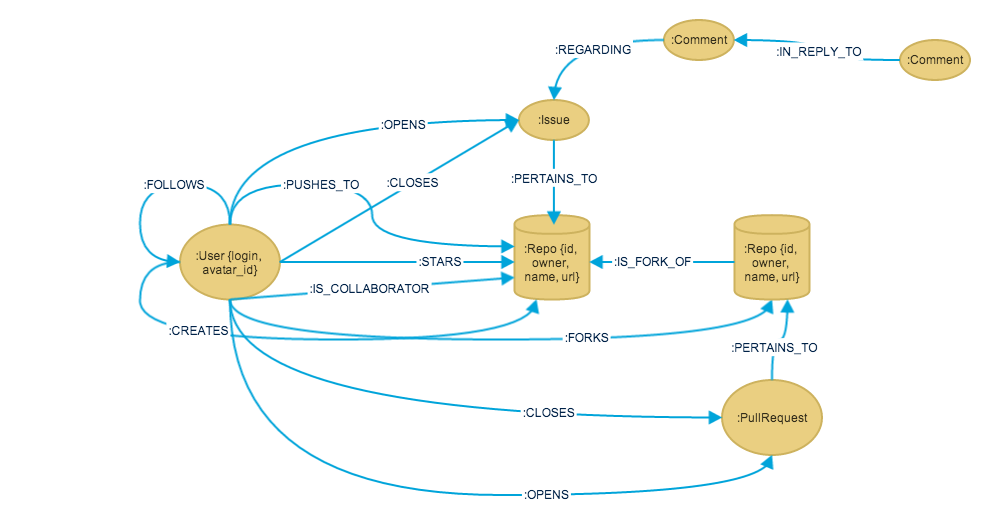
\includegraphics[width=0.75\textwidth]{images/githubdatamodel.png}
  \caption[GitHub graph data model]{GitHub data model as a labeled property graph.}
  \label{github_data_model}
\end{figure}

GitHub \footnote{\url{http://github.com}} is an online social collaboration network built around the Git version control system. GitHub allows software developers to share and collaborate on software projects. Many open-source software projects are hosted on GitHub and use GitHub as their primary development and distribution platform. GitHub also has a social component: users are able to \textit{follow} other users to receive updates about user activity. This combination of social and collaboration components make GitHub an excellent example of a multi-modal complex network. 


\begin{figure}[ht]
\vskip 0.2in
\begin{center}
\centerline{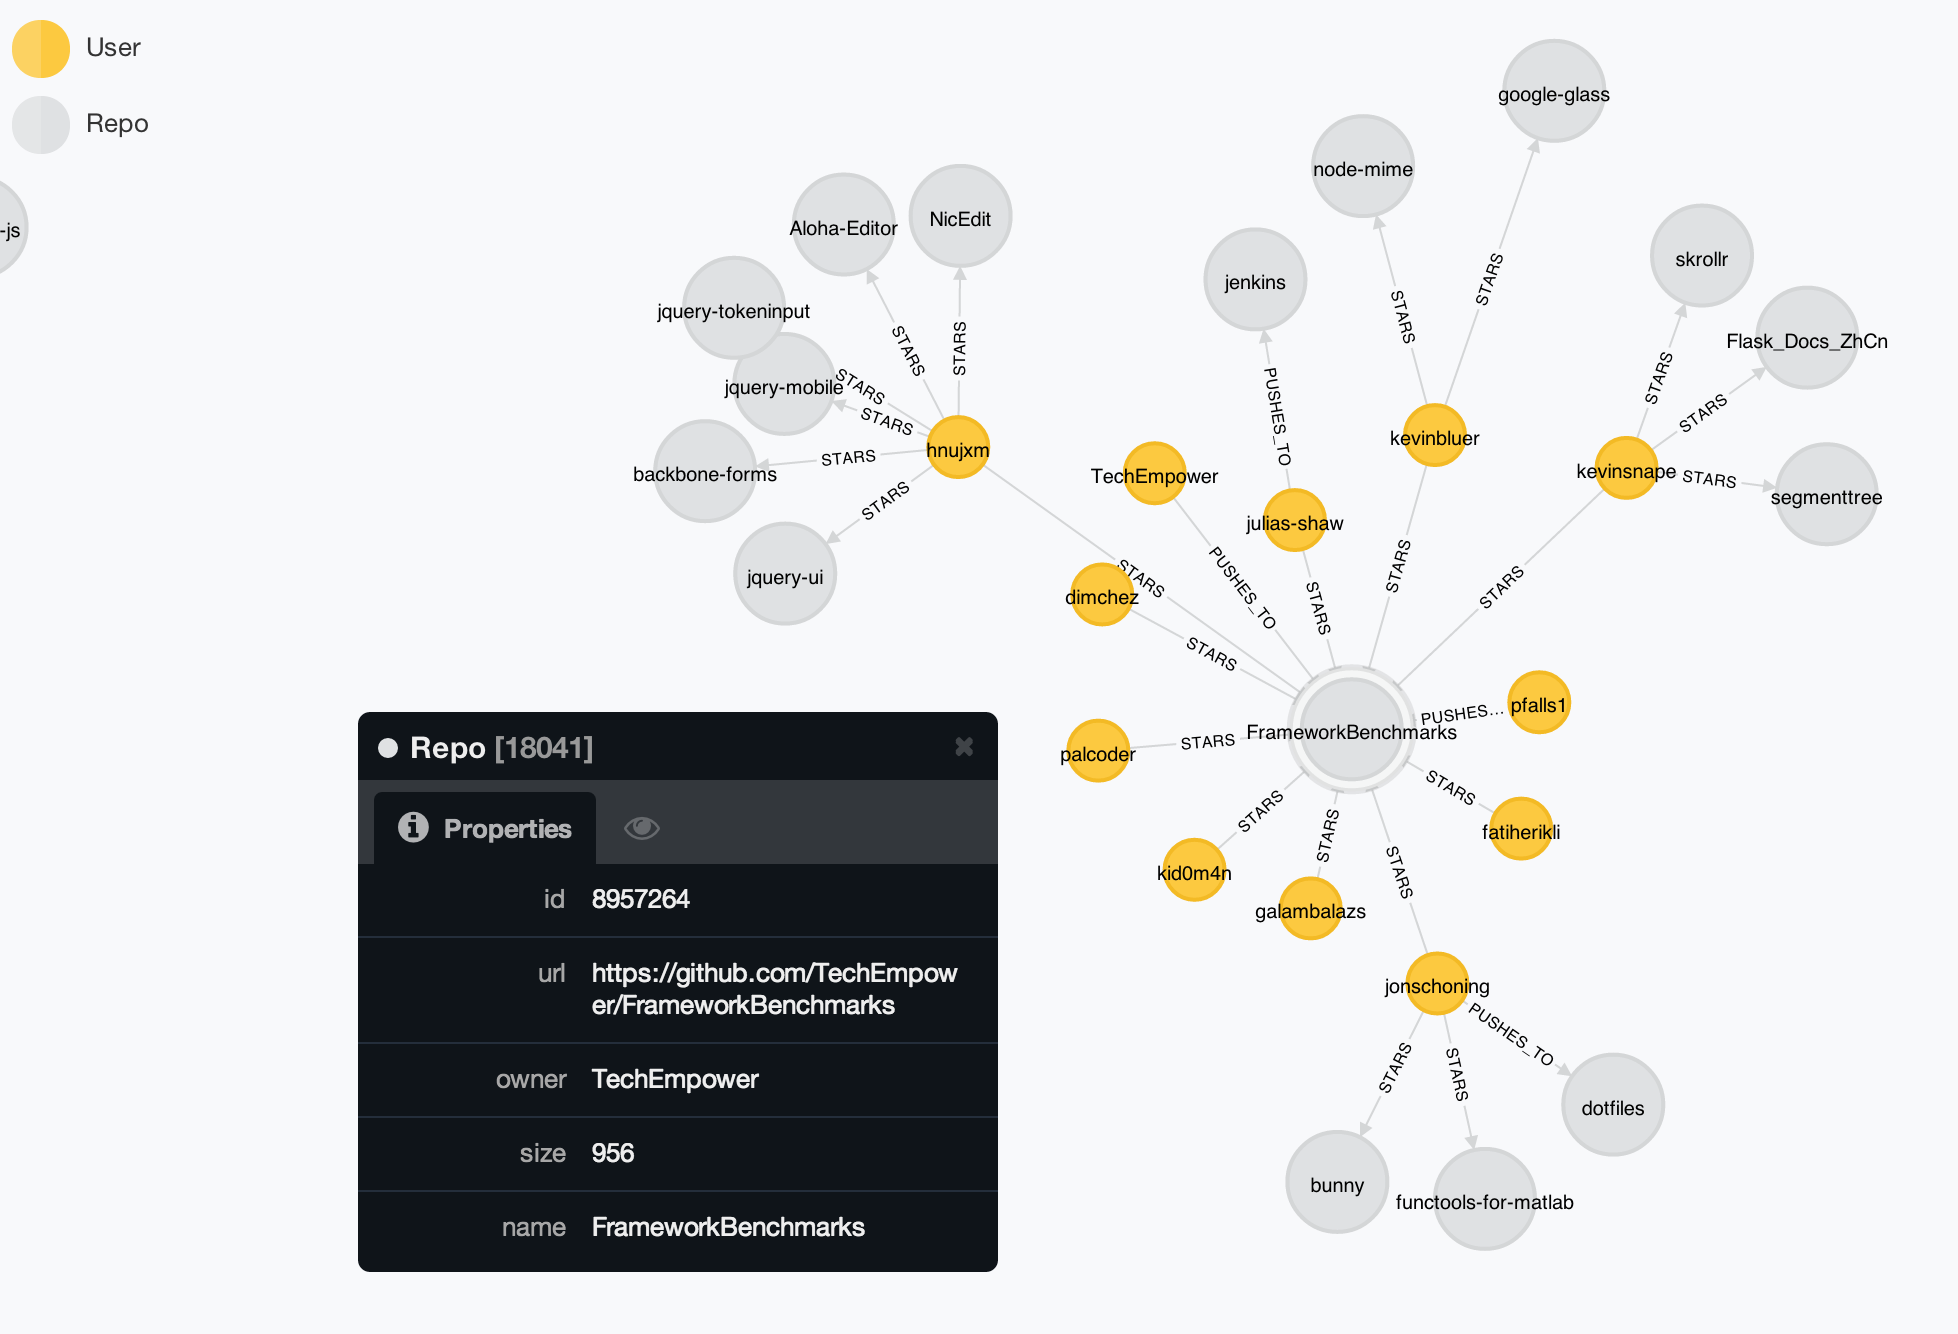
\includegraphics[width=0.75\columnwidth]{images/neo_screenshot.png}}
\caption{GitHub data model as a property graph. Screenshot from Neo4j graph database interface.}
\label{screenshot-data}
\end{center}
\vskip -0.2in
\end{figure} 


The GitHub network is multi-modal in that there are multiple nodes types (primarily Users and Repositories, or software projects) and multiple edge types (User-User follows, User-Repository Stars, etc). Figure \ref{github_data_model} shows a portion of the GitHub data modeled as a graph. This data model is quite rich, however for the purposes of this paper we will only concern ourselves with User-User \textit{:FOLLOWS} and User-Repository \textit{:STARS} edges. That simplifies the data model to that shown in Figure \ref{github_simplified_data_model}.


\begin{figure}[ht]
\vskip 0.2in
\begin{center}
\centerline{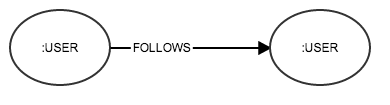
\includegraphics[width=0.3\columnwidth]{images/user_user.png}}
\caption[User-User data model]{The GitHub follow graph is a simple graph with User nodes and Follows edges.}
\label{github_simplified_data_model}
\end{center}
\vskip -0.2in
\end{figure} 

\subsection{Github Archive}
Data was collected from GitHub Archive\cite{githubarchive}, a service that maintains an archive of all public events emitted by the GitHub API\cite{github:Online}. These include events such as creation of new repositories, pushes to repositories, repository stars, and user follows. Data was collected for the time period April 1st, 2013 - April 1st, 2014. For the purposes of this project, only \textit{FOLLOWS} events were considered. This resulted in a total of 539893 users and 919489 follows. In terms of a graph, that equates to 539893 nodes and 919489 vertices between nodes.

A graph data model is used to represent this data as the data is highly connected: it is describing entities (users and repositories) and their interactions (stars, follows, pushes, etc). Figure \ref{screenshot-data} shows an example of a subgraph of user and repository nodes and the interactions among those entities, modeled as a graph.

\subsubsection{FollowEvent}
\begin{lstlisting}[style=lstStyleCpp, caption={LaTeX Typesetting By Example}, label=lstLaTeXExample]
{
  "created_at": "2013-07-11T15:03:05-07:00",
  "payload": {
    "target": {
      "id": 4602587,
      "login": "smarquez1",
      "followers": 1,
      "repos": 1,
      "gravatar_id": "42eb6556201588fa7641bf2f0bf615e6"
    }
  },
  "public": true,
  "type": "FollowEvent",
  "url": "https://github.com/smarquez1",
  "actor": "matiasalvarez87",
  "actor_attributes": {
    "login": "matiasalvarez87",
    "type": "User",
    "gravatar_id": "0ee1a5bec013545c91ad05c451fb9715",
    "name": "Matias Alvarez Duran",
    "company": "NaN Labs",
    "blog": "http://ar.linkedin.com/pub/matias-emiliano-alvarez-duran/17/39b/a96",
    "location": "Argentina",
    "email": "matiasalvarez87@gmail.com"
  }
}
\end{lstlisting}

\subsubsection{WatchEvent (Stars)}
\begin{lstlisting}[style=lstStyleCpp, caption={peep this JSON object dawg},
label=watchEventListing]
{
  "created_at": "2013-07-11T15:01:56-07:00",
  "payload": {
    "action": "started"
  },
  "public": true,
  "type": "WatchEvent",
  "url": "https://github.com/CamDavidsonPilon/Probabilistic-Programming-and-Bayesian-Methods-for-Hackers",
  "actor": "cebe",
  "actor_attributes": {
    "login": "cebe",
    "type": "User",
    "gravatar_id": "2ebfe57beabd0b9f8eb9ded1237a275d",
    "name": "Carsten Brandt",
    "company": "cebe.cc",
    "blog": "http://cebe.cc/",
    "location": "Berlin, Germany",
    "email": "mail@cebe.cc"
  },
  "repository": {
    "id": 7607075,
    "name": "Probabilistic-Programming-and-Bayesian-Methods-for-Hackers",
    "url": "https://github.com/CamDavidsonPilon/Probabilistic-Programming-and-Bayesian-Methods-for-Hackers",
    "description": "aka \"Bayesian Methods for Hackers\": An introduction to Bayesian methods + probabilistic programming with a computation/understanding-first, mathematics-second point of view. All in pure Python ;)  ",
    "homepage": "http://camdavidsonpilon.github.io/Probabilistic-Programming-and-Bayesian-Methods-for-Hackers",
    "watchers": 3353,
    "stargazers": 3353,
    "forks": 444,
    "fork": false,
    "size": 1264,
    "owner": "CamDavidsonPilon",
    "private": false,
    "open_issues": 21,
    "has_issues": true,
    "has_downloads": true,
    "has_wiki": true,
    "language": "Python",
    "created_at": "2013-01-14T07:46:28-08:00",
    "pushed_at": "2013-07-04T17:08:47-07:00",
    "master_branch": "master"
  }
}
\end{lstlisting}

\subsection{Data munging}
The data from GitHubArchive is available in streaming JSON format and includes all public events generated from the GitHub event API \cite{github:Online} for a given time period. The one year of data collected for this project resulted in several thousand JSON files, each several megabytes in size resulting in a raw dataset of several hundred gigabytes. As this project is only concerned with the user-user {\textit FOLLOWS} relationship, the data is parsed using a Python script to filter for only those {\textit FOLLOWS} events. For further efficiency, the data is reduced to an anonymized edgelist format:
\begin{verbatim}
    1	2
    3	4
    5	6
    7	8
    9	10
    11	12
    11	13
    14	15
    16	17
    18	19
    ...
\end{verbatim}
This allows for the dataset to be anonymized using only arbitrary user ids and stored as compactly as possible. In the above example (and in the context of a directed graph) the first column corresponds to the source node and the second column the destination node. So the sample above represents: user 1 follows user 2, user 3 follows user 4, ...

This edgelist file is then used to populate a Neo4j graph database instance, using only the minimal information necessary to implement our link prediction system. 

\begin{table}[ht]
\centering
\small\renewcommand{\arraystretch}{1.4}  
\rowcolors{1}{tablerowcolor}{tablebodycolor}
%
\captionabove[GitHub network descriptive statistics]{Here we see the most "central" Users per their PageRank rankings. This is based on the graph created by user-user follows edges.}
\label{follow_pagerank_table}
\begin{tabularx}{0.7\textwidth}{lXXX}
\hline
\rowcolor{tableheadcolor}
 & Count \\
\hline
Nodes (users) & 539893  \\
Edges (:FOLLOWS relationships) & 919489 \\
Mean degree & 3.4 \\
Standard deviation of degree & 30.3 \\
\hline
\hline
\end{tabularx}
\end{table}


\subsection{Data Analysis}

\begin{table}[ht]
\centering
\small\renewcommand{\arraystretch}{1.4}  
\rowcolors{1}{tablerowcolor}{tablebodycolor}
%
\captionabove[PageRank for User-User follows]{Here we see the most "central" Users per their PageRank rankings. This is based on the graph created by user-user follows edges.}
\label{follow_pagerank_table}
%
\begin{tabularx}{0.4\textwidth}{lXXX}
\hline
\rowcolor{tableheadcolor}
User & PageRank \\
\hline
funkenstein& 413.14 \\
mojombo & 300.01 \\
torvalds & 248.21 \\
rippleFoundation & 220.29 \\
visionmedia & 140.52 \\
paulirish & 129.59 \\
BYVoid & 114.29 \\
schacon & 112.17 \\
JakeWharton & 110.55 \\
defunkt & 106.86 \\
mattt & 99.38 \\
worrydream & 87.33 \\
hakimel & 83.05 \\
pjhyett & 80.89 \\
addyosmani & 80.59 \\
mbostock & 75.63 \\
mdo & 70.40 \\
LeaVerou & 66.92 \\
tekkub & 62.24 \\
nf & 60.93 \\
\hline
\end{tabularx}
\end{table}




\begin{table}[ht]
\centering
\small\renewcommand{\arraystretch}{1.4}  
\rowcolors{1}{tablerowcolor}{tablebodycolor}
%
\captionabove[PageRank for User-Repository stars]{Top 20 central GitHub repositories by PageRank.}
\label{follow_pagerank_table}
%
\begin{tabularx}{0.8\textwidth}{lXXX}
\hline
\rowcolor{tableheadcolor}
Repository & PageRank \\
\hline
\url{https://github.com/vhf/free-programming-books} & 455.07 \\
\url{https://github.com/twbs/bootstrap} & 335.46 \\
\url{https://github.com/jquery/jquery} & 289.42 \\
\url{https://github.com/resume/resume.github.com} & 251.99 \\
\url{https://github.com/mandatoryprogrammer/Octodog} & 233.41 \\
\url{https://github.com/angular/angular.js} & 202.18 \\
\url{https://github.com/mbostock/d3} &149.55 \\
\url{https://github.com/torvalds/linux} & 133.48 \\
\url{https://github.com/FortAwesome/Font-Awesome} & 121.47 \\
\url{https://github.com/twitter/bootstrap} & 111.42 \\
\url{https://github.com/laravel/laravel} & 106.75 \\
\url{https://github.com/papers-we-love/papers-we-love} & 102.25 \\
\url{https://github.com/joyent/node} &101.27 \\
\url{https://github.com/rethinkdb/rethinkdb} & 92.34 \\
\url{https://github.com/neovim/neovim} & 91.52 \\
\url{https://github.com/libgit2/libgit2} & 90.99 \\
\url{https://github.com/rogerwang/node-webkit} & 88.23 \\
\url{https://github.com/github/gitignore} & 88.08 \\
\url{https://github.com/dypsilon/frontend-dev-bookmarks} & 86.73 \\
\url{https://github.com/zurb/foundation} & 84.25 \\
\hline
\end{tabularx}
\end{table}
